%!TEX root = ../main_text.tex

\chapter{Metodologia Proposta} \label{chap:met2}
   %bla bla bla
   Apresentado o problema de particionamento, sua importância, será apresentado uma abordagem para o projeto de sistemas computacionais \wearables\ e aplicações deste em sistemas hipotéticos.

   % Tem vários trabalhos, mas sem wearable
   Como foi possível perceber no Capítulo Trabalhos Relacionados (Capítulo \ref{chap:relacionados}), existem vários trabalhos em sistemas computacionais embarcados, entretanto, nenhum que abordasse o tema para \wearables.
   %justificativa de bateria e die
   Partindo deste pressuposto, esta pesquisa propõe o estudo de dispositivos \wearables\ e a aplicação de técnicas de particionamento a fim de obter um desempenho melhor para estes.

   % pesquisa com fourier
   %Sendo assim, será realizado uma pesquisa de particionamento sobre algoritmos comumente utilizados em sistemas \wearables\ de forma a verificar seus gastos energéticos e recursos utilizados em \hardware, como por exemplo o cálculo da Transformada de Fourier, fórmula utilizado em situações cabíveis em dispositivos \wearable\ como análise, filtros, reconstrução e compressão de imagens, por exemplo.

   %metodologia
   A metodologia proposta baseia-se em procedimentos que utilizam as técnicas descritas neste documento.
   No Capítulo \ref{chap:design} foi descrito os principais métodos utilizados neste trabalho, e ao final foi apresentado um procedimento na qual a metodologia usará como base.
   O método consiste unicamente na organização dos conceitos discutidos a fim de obter uma análise sistemática do projeto e assim, realizar o particionamento a procura de melhorias.
   A diferença entre a análise metodológica de um exemplo hipotético e de um dispositivo real é que com o real, todas as principais funções do dispositivo são consideras e assim, a quantidade de procedimentos a serem considerados para o particionamento \hs\ seria maior, criando um leque maior de possibilidade para análise.
   Assim, para demonstração da metodologia, será realizada sua aplicação para a análise de dois dispositivos \wearables\ hipotéticos descritos nas Seções~\ref{sec:hip1} e \ref{sec:hip2} a seguir.


   \section{\Wearable\ Hipotético 1: Mão Biônica} \label{sec:hip1}

      \paragraph{Apresentação}
         % Exemplificação teórica
         %A seguir será apresentado uma situação hipotética na qual a metodologia do tema pesquisado seria aplicada.
         % porque do problema
         Como já é de conhecimento, o ser humano, bem como todos os outros animais, usa de seus músculos corporais para as tarefas cotidianas como andar, comer, etc.
         Com o estímulo ordenado dos músculos, é possível realizar atuações até mais complexas como segurar um objeto pelas mãos ou mesmo, ter controle sobre um automóvel ou realizar uma performance artística/musical.
         %Todos estes necessitam de uma ordenação e coordenação dos movimentos realizados.
         %apresentação do wearable
         Assim, uma situação de uso de \wearable\ é, ao invés do usuário utilizar de suas próprias mãos para realizar alguma atividade como a de segurar um objeto, com a adição de um sistema \wearable, seria possível intermediar a atuação final (tomar algo pelas mão), com a leitura da tensão elétrica muscular do usuário ao longo do tempo, a fim de substituir a atuação de sua mão por meio de atuadores mecânicos artificiais, como mostra a Figura~\ref{fig:maobionica}.

         \begin{figure}[h] \centering
            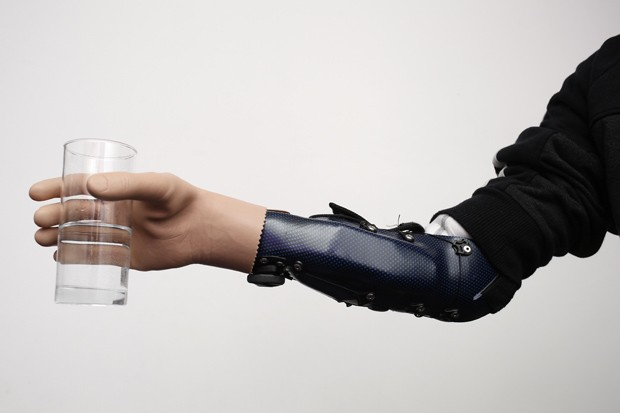
\includegraphics[width=0.7\textwidth]{img/maobionica.jpg}
            \caption{Demonstração de uma mão biônica. Fonte: \url{https://goo.gl/96PURB} Acesso: 30/07/2017.}
            \label{fig:maobionica}
         \end{figure}

         %técnico
         Descrevendo-o de uma forma mais técnica, o \wearable\ deve ser capaz de realizar leituras eletromiográficas%
         \footnote{Técnica na qual realiza o monitoramento de atividades elétricas das células musculares.},
         interpretá-las de acordo com um pretexto e realizar a atuação.
         Um pseudo-algoritmo é apresentado em Algoritmo~\ref{alg:wearable1}.
         %
         % particionamento no wearable apresentado
         Pode-se supor que o dispositivo foi inteiramente construído em uma solução em \software\ com a justificativa de projeto de uma construção mais simples.
         Assim sendo, o particionamento \hs\ entra com o papel de analisar o projeto a fim de buscar por combinações de particionamento que apresentem melhorias em performance ou no gasto energético ao estado atual.
         A análise é importante mesmo para projetos que já possuam aceleradores em \hardware\ em seu projeto pois a verificação atua como uma forma de validação e confirmação de sua performance como uma solução aproximada do ótimo.

         \begin{algorithm}[h]
            \SetKwData{md}{matrix\_data}
            \SetKwData{mdp}{matrix\_data\_preprocessed}
            \SetKwData{eb}{buffer\_state}
            \SetKwData{ea}{state\_before}
            \SetKwData{sx}{sensor$_i$}
            \SetKwFunction{leSensores}{reads\_sensors}
            \SetKwFunction{preprocess}{pre\_process}
            \SetKwFunction{process}{processes}
            \SetKwFunction{atuacao}{operates}
            \SetKwFunction{bu}{backup}

            \KwIn{sensors reads.}
            \KwOut{acting.}
            \BlankLine

            \Begin{
               \BlankLine
               \tcp{statements}
               \sx\tcp*{$i$ information's source}
               \md\tcp*{data's matrix before handling}
               \mdp\tcp*{data's matrix after handling}
               \eb\tcp*{last state applied and current}
               \ea\tcp*{generated state to be compared}
               \BlankLine

               \While{wearable mode on}{
                  \md $\leftarrow$ \leSensores{\sx}\;
                  \mdp $\leftarrow$ \preprocess{\md}\;

                  \BlankLine

                  \tcp{process the datas}
                  \If{\eb $\leftarrow$ \process{\mdp} $\ne$ \ea}{
                     \tcp{operates}
                     \ea $\leftarrow$ \eb\;
                     \atuacao{\ea}\;

                     \BlankLine
                     \bu{}\tcp*{saves the data persistently}
                  }
                  \BlankLine
               }
            }

            \caption{\Wearable\ 1 - Procedimentos realizados pelo dispositivo \wearable\ denominado Mão Biônica.}
            \label{alg:wearable1}
         \end{algorithm}

         Suponha então que deseja-se realizar uma avaliação de particionamento \hs\ de um dispositivo \wearable\ que atua por meio de tais sinais eletromiográficos.
         %O primeiro passo a ser realizado é a construção do grafo de chamada do projeto, exibido no próximo tópico.

      \paragraph{Análise Usando \Profile}
         O primeiro procedimento a ser realizado para a obtenção de informações de projeto e execução do programa é com a execução de um \software\ que faça o seu \profile.
         Ao realizar esta tarefa, obtêm-se resultados de tempo de execução dos principais procedimentos do projeto, listados de forma ordenada por tempo gasto, como já descrito na Seção \ref{sec:profile}.
         
         Feito esta análise, é construído o grafo de chamada de acordo com a especificação de funcionamento do projeto.

      \paragraph{Grafo}
         A partir do pseudo-algoritmo dado e da análise \profile, é possível gerar o grafo de chamada, exibido pela Figura~\ref{fig:graph_w1}.
         %explicação grafo
         Como descrito na Seção \ref{sec:GCF}, é realizado uma análise no projeto verificando os códigos e funções, gerando o seu respectivo grafo de chamada.
         %Como este é um exemplo hipotético, gerou-se um grafo mais simples, mas que ainda representa o real funcionamento do dispositivo.

         \begin{figure}[h] \centering
            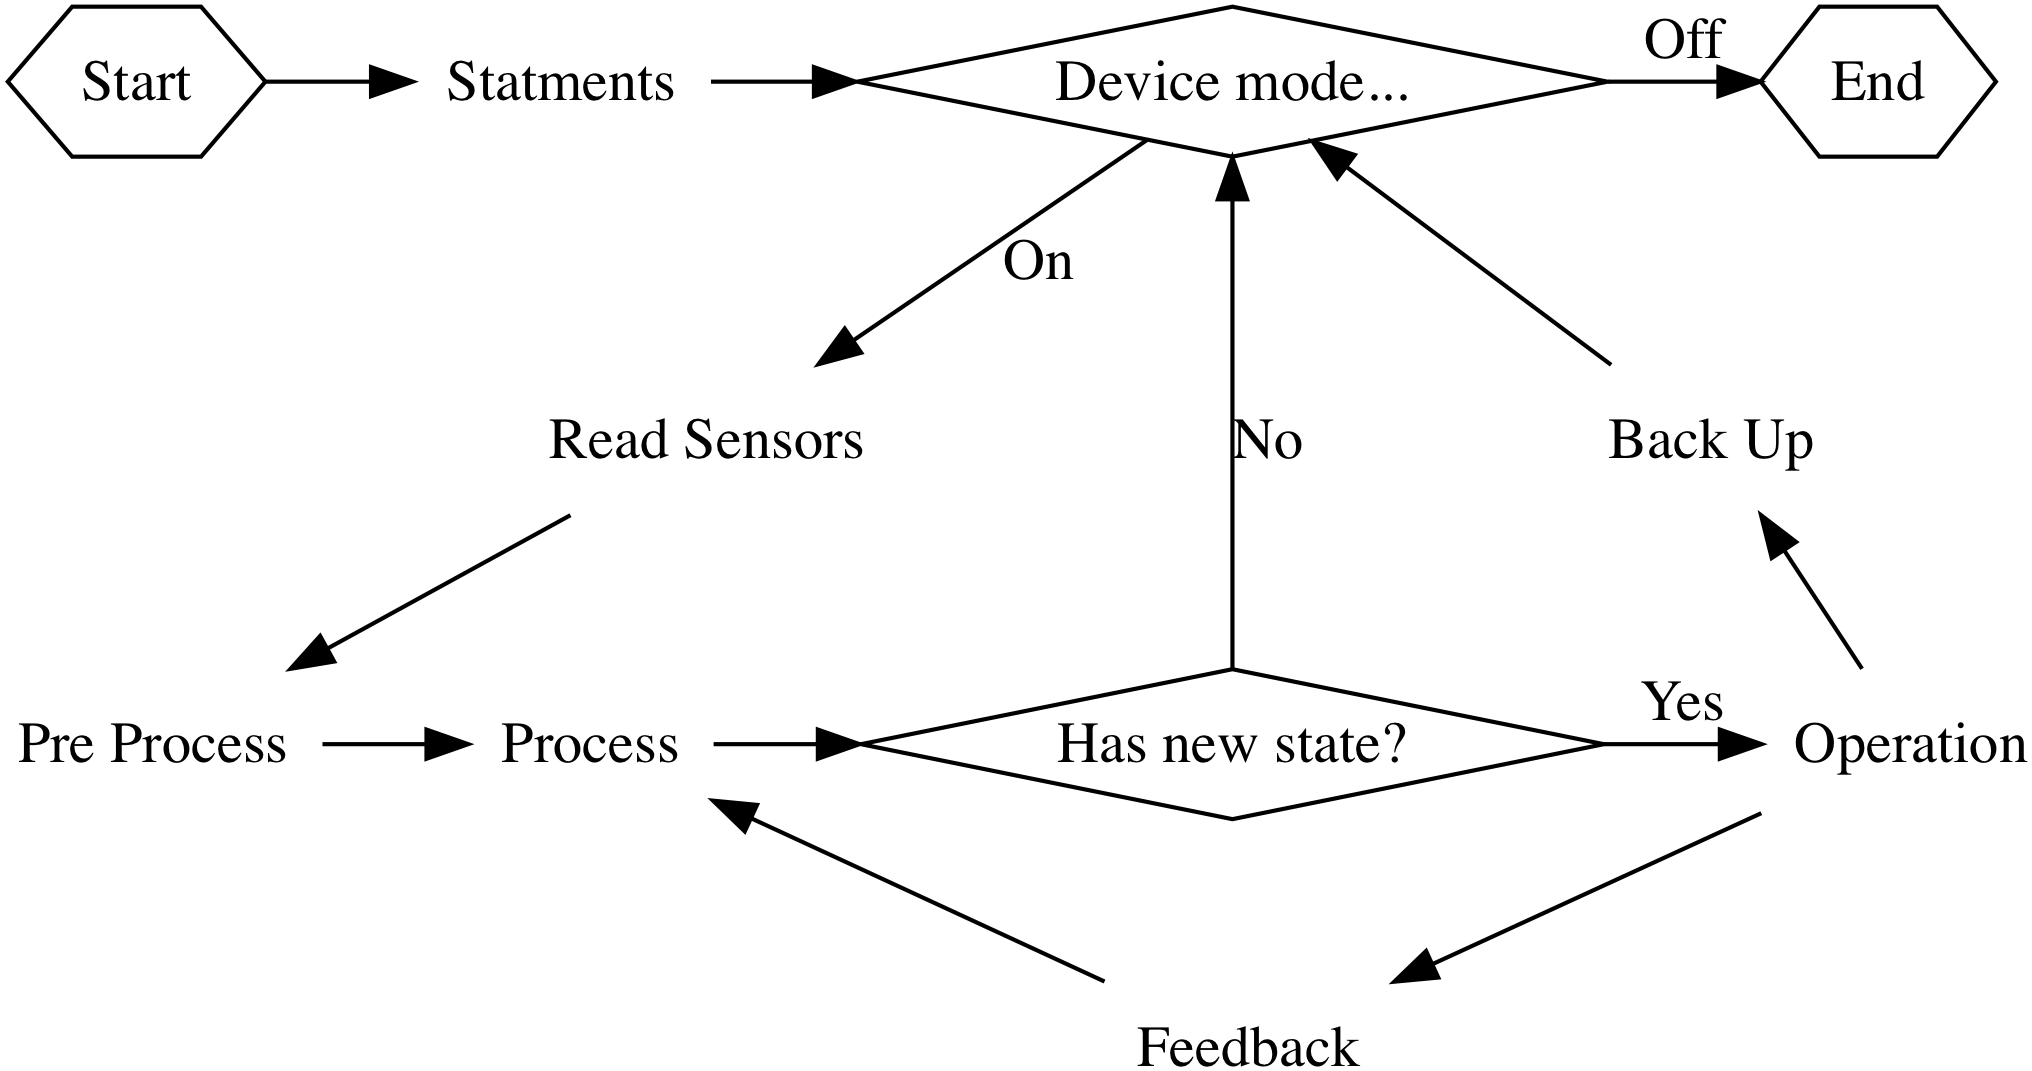
\includegraphics[width=0.9\textwidth]{img/graph_wearable.png}
            \caption{Exemplificação de um grafo de chamada para o exemplo.}
            \label{fig:graph_w1}
         \end{figure}

         %explicando o grafo
         %start
         O processo representado pelo grafo da Figura~\ref{fig:graph_w1} inicia-se pelo estado de formato hexágono com etiqueta \textit{start}.
         %statment
         Ao iniciar o dispositivo, é realizado as inicializações de ambiente, definidas pelo estado seguinte \textit{statments}, realizando todas as definições prévias para seu uso.
         Este processo é unicamente para inicialização do equipamento, redefinindo todos os estados da última operação ou de um estado específico de inicialização.
         %if 1
         Em seguida, tem-se o primeiro losango indicando uma verificação de estado.
         Neste, verifica-se se o dispositivo entrou-se em modo de desligamento, se sim, desligando-o de forma segura.
         %process
         Caso contrário, realiza leituras eletromiográficas, o pré-processamento delas e em seguida o processamento dos dados.
         %if 2
         Após processado, é verificado se existe um novo estado de acordo com os valores lidos.
         %operacao
         Se este novo estado é distinto do anterior, então o dispositivo deve realizar a operação de alteração da atuação para este novo, além do armazenamento deste em forma persistente para inicialização, caso estabelecido e o processo é reiniciado na verificação de de dispositivo ligado.
         Neste também é realizado a leitura de \textit{feedback} da atuação retornando-o para o processamento para avaliar o erro e gerar uma resposta para tal.

         % grafo hipotético vs real
         O grafo gerado deste exemplo apresentado é uma solução simplista pelo fato de ser inteiramente hipotético.
         Com um exemplo real, seria possível ter um detalhamento maior no grafo, já que este teria informações suficientes sobre os procedimentos do dispositivo para compreendimento.

         Ao concluir a construção do grafo do sistema \wearable\ e analisá-lo, consegue-se ter conhecimento de grupos procedurais importantes e assim, consequentemente separá-las em módulos.
         %Como \wearables\ baseiam-se em avaliação, interpretação e ação, será aplicada uma identificação de grupo para facilitar o entendimento de cada módulo do dispositivo.
         Foram denominados três grupo para a organização dos procedimentos, sendo eles Leitura, Processamento e Atuação, e serão descritos a seguir.

         \begin{description}
            \item [Módulo de Leitura:]
            A leitura é realizada por meio de um sensor muscular na qual obtém sinais eletromiográficos, ou seja, um sensor de eletromiograma.

            Não só como a leitura mas a interpretação dos sinais elétrico depende diretamente da natureza dos dados sensoriais obtidos pelo eletromiograma, um pré-processamento de tais dados é um fator está relacionado diretamente com a obtenção de informação do conjunto de dados.
            Então, supondo que o dispositivo \wearable\ também necessite de um pré-processamento dos dados para filtragem e preparação para o processamento central de fato, este estaria incluso dentro do módulo de leitura, enviando-os em seguida para o processamento central.
            
            O grupo será composto pelos procedimentos: \texttt{Statments}, \texttt{Read Sensors} e \texttt{Pre Process}.

            \item [Módulo de Processamento Central:]
            Com os dados já trabalhados para serem utilizados de forma mais clara, o próximo passo a ser realizado é a interpretação destes de acordo com um pretexto pré-estabelecido pelo projetista e assim tomar uma decisão sobre este.
            Dessa forma, é realizado uma verificação de padrões do conjunto de dados recebido e a alteração de estado de atuação caso necessário.

            Caso exista tal mudança, especificar qual e passar isso para o próximo módulo, a atuação.
            Caso contrário realiza novas leituras de dados, já que não obteve nenhuma alteração de estado de atuação.

            Para o projeto ser mais responsivo, seria ideal obter também um \textit{feedback} relativo à atuação, criando uma correlação mais precisa entre os dados lidos de sensores musculares com o estado do atuador e sua atuação.
            O \textit{feedback} seria relacionado à completude da atuação, verificando se a atuação foi realmente executada como esperado e, caso negativo, encontrar o valor de erro para a sua tentativa de correção, processamento a ser realizado neste módulo.
            
            Composto pelos procedimentos: \texttt{Process} e \texttt{feedback}.

            \item [Módulo de Atuação:]
            Meio no qual realiza-se a atuação, segundo implicação oriunda do processamento central.

            Neste, também seria realizado as leituras de \textit{feedback}, enviando-os para o módulo de processamento central.
            
            Composto pelas funções: \texttt{Operation} e \texttt{Back Up}.
         \end{description}

      Após feito o \profile\ e o desenvolvimento do grafo, deve-se verificar quais procedimentos são candidatos a serem sintetizados para análise de performance.
      Procedimentos que realizam cálculos matemáticos repetitivos, ou que são executados ocasionalmente são excelentes candidatos já que pode-se utilizar os recursos de \hardware\ para o processamento com maior vazão de dados ou o acionamento e desligamento do recursos quando não utilizado, respectivamente às situações apresentadas.

      \paragraph{Análises de Síntese}
         Construído o grafo e verificado os candidatos ao particionamento por meio do \profile, realiza-se então a sintetização de todos os procedimentos candidatos bem como suas análises de uso de recursos e performance.
         
         Todos os procedimentos do projeto apresentado são candidatos a serem sintetizados e analisados.
         São procedimentos que também necessitam de resposta imediata ao estímulo dado, aproximando ao máximo à uma atuação instantânea realizada pelos membros musculares naturais.
         Isso pois, todos os procedimentos podem ser executados sem a presença de um microcontrolador, usando recursos de uma máquina de estados para controle por exemplo.
         
         Dessa forma, como são candidatos, serão sintetizados, analisados e comparados com os procedimentos realizados via \software\ por meio de um microcontrolador.
         
      \paragraph{\textit{Solver}}
         Obtida as análises de cada componente em nível de \software\ e \hardware, utiliza-se de \textit{solvers} para encontrar uma solução boa.
         
         No Capítulo \ref{chap:relacionados}, existem inúmeras aplicações que utilizam desde métodos exatos baseado em programação inteira linear até metaheurísticas.
         Dessa forma, após a aplicação do método \textit{solver}, obteremos um particionamento solucionado pelo solver de acordo com as restrições de recursos impostas.


   \section{\Wearable\ Hipotético 2: Capacete para Segurança de Ciclistas} \label{sec:hip2}
      \paragraph{Apresentação}
         Outro exemplo de \wearable\ e suas análises está em propor um capacete desenvolvido para a segurança de ciclistas.
         O hipotético propósito deste seria fornecer um auxílio para a segurança do usuário, junto com dados estatísticos de corrida com a bicicleta.
         
         O equipamento seria utilizado para verificar situações na qual um veículo estaria se aproximando do usuário pela suas costas de forma a gerar uma colisão, local sem visibilidade constante pelo ciclista.
         Dessa forma, o capacete poderia avisar o ciclista para manter cuidado e tomar uma atitude segura enviando alguma informação para seu \textit{smartphone} ou para algum dispositivo \textit{wearable} acoplado ao seu corpo como uma pulseira.
         Ambos dispositivos poderiam passar a informação para o ciclista por meio de estímulos visuais ou físicos como luzes ou vibrações ou, pensando num equipamento mais tecnológico, um aviso em um óculos com realidade aumentada, por exemplo.
         
         Como já dito, além da prevenção de acidentes, o equipamento poderia ainda suportar procedimentos que realizem a obtenção e envio de dados de atividades físicas do usuário como distância percorrida, tempo de atividade e na qual, após o processamento dos dados, a geração de informações como velocidade média, estimação de calorias queimadas, entre outras.
         Isso, enviando para um aplicativo no seu telefone móvel por meio de uma conexão sem fio.

         O projeto, em termos técnicos, seria composto de sensores capazes de realizar a verificação de objetos volumosos e sua distância em relação ao ponto atual do ciclista.
         Ao avistar um objeto aproximando, por meio de uma conexão sem fio, o capacete enviaria um pacote de notificação para os dispositivos acoplados ao corpo do usuário avisando-o que está em uma situação de perigo.
         Além de tais dispositivos, o capacete poderia reagir também com sinais luminosos situados nele próprio, a fim de alertar o ciclista e/ou também o motorista mostrando que existe um algo em sua frente que na qual, necessita de sua atenção para não haver uma colisão.
         
         Já os dados de atividade física podem ser obtidos por meio de acelerômetros, giroscópios, GPS, RTC, na qual permitem a interpretação dos dados por meio de cálculos, gerando informações de posicionamento, orientação, velocidade, tempo, além de gasto energético, velocidade média percorrida e até um sistemas de conquista de metas.
         É possível desenvolver um sistema na qual relacione todos os sensores como o exemplo de que o sensor de risco só seja ativado quando o ciclista esteja se movimentado, situação na qual utiliza os sensores de distância e acelerômetro.
         Os dados de todos os sensores seriam gravados em uma memória não volátil para acesso e sincronização com um \textit{smartphone} futuramente.
   
         A seguir será exibido vários procedimentos responsáveis por demonstrar a execução do dispositivo.         
         O primeiro, Algoritmo~\ref{alg:wearable2_leituras}, exibe o procedimento para leitura de sensores e o armazenamento de tais informações em memória não-volátil.
         Caso verificado que existe uma situação de risco acontecendo por meio da leitura, também será realizado o envio de um sinal de interrupção para o controlador a fim de que os procedimentos de aviso sejam realizados.
   
         \begin{algorithm}[h]
            \SetKwData{data}{datas}
            \SetKwData{typew}{type\_warning}
            \SetKwData{sx}{sensor$_i$}
            \SetKwFunction{leSensores}{reads\_sensors}
            \SetKwFunction{preprocess}{pre\_process}
            \SetKwFunction{process}{processes}
            \SetKwFunction{atuacao}{operates}
            \SetKwFunction{finterrupt}{does\_interruption}
            \SetKwFunction{bu}{backup}
            
            \BlankLine
            \KwIn{sensors reads.}
            \KwOut{backups and interruptions signals.}
            \BlankLine
   
            \Begin{
               \tcp{statements}
               \sx\tcp*{$i$ information's source}
               \data\tcp*{data's matrix before handling}
               \typew\tcp*{type of warning to do to user}
               \BlankLine
   
               \While{wearable mode on}{
                  \data $\leftarrow$ \leSensores{\sx}\;
                  \BlankLine
   
                  \tcp{process the datas}
                  \typew $\leftarrow$ \process{\data}\;
                  
                  \BlankLine
                  \If{\typew $=$ dangerous}{
                     \finterrupt{\typew}\;
                  }                  
                  
                  \BlankLine
                  \bu{\data}\;
   
                  \BlankLine
               }
               \BlankLine
            }
   
            \caption{\Wearable\ 2 - Procedimento que realiza leituras de sensores e armazena seus dados em memória não-volátil.}
            \label{alg:wearable2_leituras}
         \end{algorithm}
         
         Dessa forma, o Algoritmo~\ref{alg:wearable2_leituras}, na linha 6, realiza leitura dos sensores e em seguida verifica se existe alguma gravidade na situação.
         Se positivo, gera o sinal de interrupção.
         Como esse módulo é um módulo independente e gerador de interrupções, ao realizar uma, não necessita de criar-se um bloqueio em seus procedimentos. 
         Isso significa que o módulo poderá continuar com suas instruções de ler, analisar e gravar os dados, independente do controlador estiver ou não com interrupção.
         
         Após o controlador receber a interrupção, inicia-se o processo do Algoritmo~\ref{alg:wearable2_interrupcao} para tratá-la.
         A função \texttt{does\_interruption} é estimulada sempre que um sinal de interrupção é ativado ou mantido ativo.
         %buffer
         Após iniciada, tipo da interrupção é gravado numa variável auxiliar com nome \texttt{buffer\_type\_warning}.
         Isso é importante pois, caso a interrupção seja retirada no meio da função, não permita a possibilidade de um dispositivo realizar o alerta e outro não, criando uma confusão no compreendimento do usuário sobre sua situação.
         Como já dito, o processo de alerta ficará ativo enquanto a interrupção estiver ativada e assim, como exibido na linha 4, o procedimento continuará em repetição enquanto o valor não ser alterado, na linha 10.
         %conexao
         O primeiro passo a se fazer ao receber a interrupção é verificar se o capacete possui conexão sem-fio com os equipamentos que possuem suporte (como o \textit{smartphone} e o \textit{wearable}).
         Se sim, envia sinal do tipo de interrupção para os dispositivos para que eles façam a parte deles.
         %leds
         Como é possível que nenhum dispositivo esteja conectado, foi idealizado também uma forma de aviso integrado ao capacete, a fim de não ficar  à mercê desses para manter a segurança do ciclista.
         Dessa forma, o dispositivo também contaria com \textit{leds} na qual seriam ativados quando estivesse em uma situação de risco, com é exibido na linha 9.
         
         Ao final do Algoritmo~\ref{alg:wearable2_interrupcao}, quando a interrupção é retirada, o \texttt{while} da linha 4 é tido como falso e assim, na linha 12, é realizado o término da interrupção em todos os dispositivos voltando para o estado normal.

         \begin{algorithm}[h]
            \SetKwProg{Fn}{Function}{ do}{end}
            \SetKwFunction{inter}{is\_there\_interruption\_yet}
            \SetKwData{typew}{type\_warning}
            \SetKwData{btypew}{buffer\_type\_warning}
            \SetKwFunction{startInterrupt}{does\_interruption}
            \SetKwFunction{finishInterrupt}{finishes\_interruption}
            \SetKwFunction{conexao}{verifies\_connection}
            \SetKwFunction{smartphone}{tries\_send\_to\_smartphone}
            \SetKwFunction{fwearable}{tries\_send\_to\_wearable}
            \SetKwFunction{leds}{does\_leds\_warning}
            
            \BlankLine
            \KwIn{interruption info.}
            \KwOut{interruption warnings.}

            \BlankLine            
            
            \typew\tcp*{interruption signal}
            \BlankLine            
            
            \Fn{\startInterrupt}{

               %\BlankLine
               \btypew $\leftarrow $ \typew\tcp*{gets the last interruption information}           
               \BlankLine            
               
               \While{\inter{\btypew}}{
               
                  \If{\conexao{}}{
                     \smartphone{\btypew}\;
                     \fwearable{\btypew}\;
                  }
                  
                  \BlankLine
                  
                  \leds{\btypew}\;
                  \btypew $\leftarrow $ \typew\tcp*{gets the last interruption information}
                  \BlankLine
               }
               \BlankLine
               
               \finishInterrupt{}\;
            }
            \caption{\Wearable\ 2 - Procedimento que realiza os procedimentos após um sinal de interrupção recebido pelo sensor de distância.}
            \label{alg:wearable2_interrupcao}
         \end{algorithm}         
         
         Por fim, tem-se o Algoritmo~\ref{alg:wearable2_control} que fica responsável dos módulos que necessitam de controle para funcionamento.
         Isso é necessário em procedimentos de sincronização e controle, sendo que neste caso é a sincronização dos dados de atividades obtidas pelos sensores para o aplicativo no \textit{smartphone}.
         
         
         \begin{algorithm}[h]
            \SetKwData{menu}{menu}
            \SetKwData{data}{datas}
            \SetKwData{typew}{type\_warning}
            \SetKwData{sx}{sensor$_i$}
            \SetKwFunction{bu}{backup}
            \SetKwFunction{conexao}{verifies\_connection}
            \SetKwFunction{fgets}{gets\_datas}
            \SetKwFunction{smartphone}{sends\_to\_smartphone}
            \SetKwFunction{fwearable}{wearable}
            \SetKwFunction{leds}{leds\_warning}
            \SetKwFunction{fmenu}{operation\_from\_user}
            
            \BlankLine
            \KwIn{sensors reads.}
            \KwOut{acting.}
            \BlankLine
   
            \Begin{
               \BlankLine
               %\menu $\leftarrow $ \fmenu{}\;
               \While{device mode on}{

                  \While{\conexao{}}{
                     \If{does app need fitness informations}{
                        \smartphone{\fgets{}}\;
                     }
                     
                  }               
                 
                  \BlankLine
               }
               \BlankLine
            }
   
            \caption{\Wearable\ 2 - Procedimentos para controle geral do \wearable.}
            \label{alg:wearable2_control}
         \end{algorithm}

         Tendo o projeto em mãos, realiza-se sua análise, usando primeiramente o \profile.
         
   
      \paragraph{Análise Usando Profile}
         Tal como o exemplo hipotético anterior (Seção~\ref{sec:hip1}), aplica-se o processo de análise execução neste projeto a fim de identificar procedimentos que necessitam de muitos recursos ou de um tempo maior para processamento. 
         Isso é obtido com o uso da ferramenta \profile.
      
         
      \paragraph{Grafo}
         Em seguida, tendo o projeto em mãos, realiza-se a construção de seu grafo de chamada, no qual é exibido na Figura~\ref{fig:graph_w2}. 
         
         \begin{figure}[h] \centering
            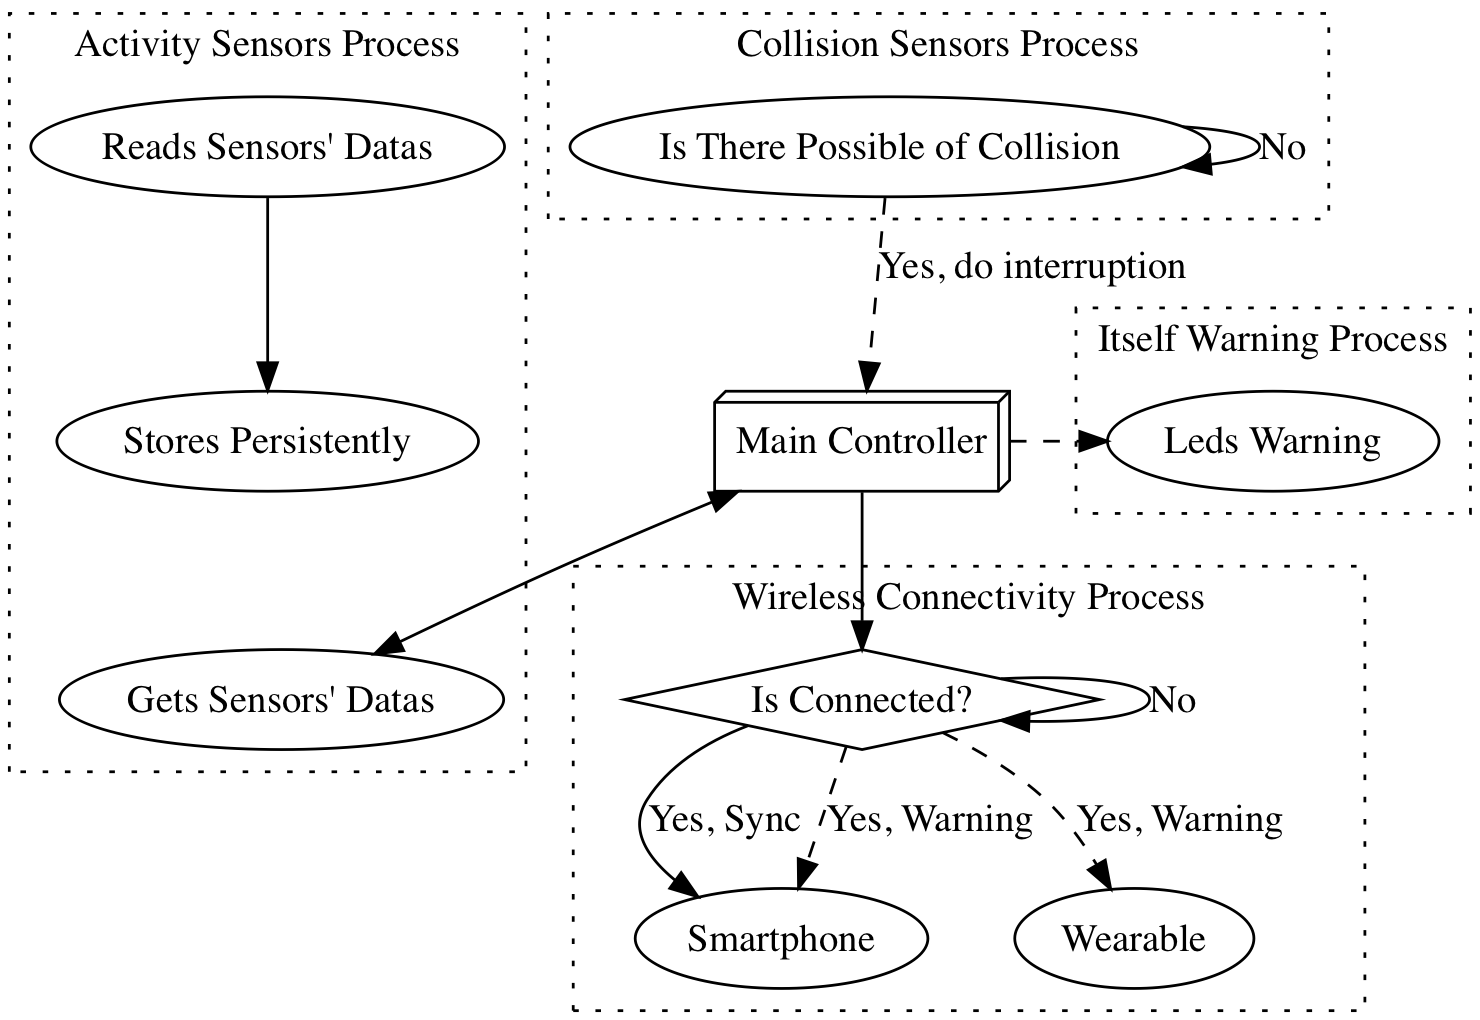
\includegraphics[width=0.9\textwidth]{img/graph_wearable2.png}
            \caption{Exemplificação de um grafo de chamada para o exemplo hipotético do capacete de segurança.}
            \label{fig:graph_w2}
         \end{figure}
         
         O grafo apresentado possui vários módulos que trabalham tanto colaborativamente quanto independente, e assim, serão mencionados e descritos separadamente a seguir para seu compreendimento.
         
         Antes de falar de cada módulo, será descrito alguns detalhes prévios.
         É possível visualizar que existem dois tipos de setas presente no grafo, isso foi feito como forma de demonstração de barramentos de comunicação na qual constituem de dados de baixa prioridade (troca de informações comuns) e dados com alta prioridade (interrupções).
         O primeiro, representado por uma seta não-tracejada ($\longrightarrow$) indica informações com baixa e o tracejado ($\dashrightarrow$), informações de alta prioridade, respectivamente.
         
         \begin{description}           
            
            \item [Sensores de Atividade:]
               Este bloco possui duas funções diferentes sendo a primeira apresenta neste tópico.
               O procedimento de leitura e armazenamento de dados sensoriais não é dependente do controlador, e com isso o processo (executado pelos procedimentos \texttt{lê sensores} e \texttt{Armazena Persistentemente}) é executado por si só.
               Dessa forma, neste processo, o capacete coleta dados e salva-os em memória constantemente a fim de criar um banco temporal de informações sem depender de um controlador para esta ação;              
               
            \item [Leitura de Dados \textit{Fitness} e Sincronização destes com o \textit{Smartphone}:]
               O outro processo, ainda relacionado ao modo anterior, parte da leitura dos dados já obtidos e envio desses do capacete para um aplicativo situado em um \textit{smartphone}.
               Este processo é já necessita de ser controlado por uma controladora e assim, foi associado com o controlador principal do projeto, para gerenciar com corretude a troca de informações;
               
            \item [Sensor de Colisão:]
               Com a leitura de dados sensoriais, outro processo também independente e de grande importância para o sistema é na análise de situações de risco e a geração de interrupções no controlador, caso exista uma.
               Esse módulo de sensoriamento de colisão compõe-se de procedimentos que realizam análises constantes de situações de risco do ciclista e enviando mensagens com interrupções para o controlador quando necessário;
               
            
            \item [Alarmes:] 
               Ao receber uma interrupção de colisão, o controlador fará logo em seguida os procedimentos de avisos nos respectivos dispositivos associados ao capacete no momento ocorrido.
               Dessa, forma o projeto constitui-se de dois tipos de avisos diferentes para o usuário, descritos a seguir:
               
               \begin{itemize}
                  \item \textbf{\textit{Alertas para Dispositivos Sem-Fio:}} 
                     Como o sistema possui comunicação sem-fio, é possível que ele envie um aviso de alerta para outros sistemas próximos a ele como \textit{smartphone} e \textit{wearables}.
                     Dessa forma, é possível que o \textit{smartphone} faça ações como vibrações ou sinais sonoros, bem como o \textit{wearable} e suas funções, a fim de alertar o usuário.
                  
                  \item \textbf{\textit{Alertas Próprio:}} 
                     Caso a comunicação não funcione, o dispositivo também terá acoplado a ele um sistema próprio na qual realizará o papel de informar o usuário sobre sua situação de risco. 
                     Este funcionará independente dos sistemas externos como meio alternativo de concluir o objetivo de informar o usuário imediatamente.
                     
               \end{itemize}
         \end{description}
         
         Com as informações obtidas até o presente momento por meio do \profile\ e o formato e fluxo do grafo, é possível identificar possíveis componentes a serem analisados em execução em \hardware, ou seja candidatos.
         
         Não é possível descrever os candidatos no exemplo hipotético pois necessita-se de informações de execução obtidas pelo \profile.
         Entretanto, podemos inferir uma lista de acordo com o propósito final de projeto e esta indução será descrita a seguir.
         Para um projeto que tenha como foco sua performance e confiabilidade, procedimentos como Verificação de Colisão e Leitura de Sensores de Atividade poderiam ser taxados como candidatos pelo fato de talvez estes se beneficiarem com a utilização de recursos em \hardware\ para a obtenção de seus objetivos.
         O procedimento de aviso integrado ao capacete também seria um candidato à análise, visto que desenvolvendo um circuito digital para seu acionamento, tem-se então respostas imediatas às interrupções geradas.
         Estes formam os componentes candidatos ao particionamento, segundo a análise induzida realizada.
         
         Por outro lado, o capacete também tem módulo de conexão sem-fio, requerendo um controlador para seu gerenciamento.
         Tal controlador deve ser capaz de certificar a conexão de dispositivos compatíveis de forma segura, realizar a transferência de informações de atividades entre o capacete e o aplicativo e tratar as interrupções com prioridade, sempre visando o consumo eficiente de energia.
         Estes, por sua vez, poderiam continuar em sua implementação em \software\ (não tornando candidatos), por se tratarem de procedimentos que não necessitam de performance, nem de grandes recursos de \hardware\ para a conclusão de suas tarefas.
         Os procedimentos compõe principalmente de leitura de dados em memória e seu envio via interface de comunicação sem-fio além do acionamento de tarefas a partir sinais interruptores.
         
         
       
      \paragraph{Análises de Síntese}
         Procedimento idêntico ao realizado com o \wearable\ hipotético da Seção~\ref{sec:hip1}.
         
         
      \paragraph{\textit{Solver}}
         Procedimento também idêntico ao realizado com o \wearable\ hipotético da Seção~\ref{sec:hip1}.
      
      
      
   \section{\Wearable\ Hipotético 3: Capacete Sensorial} \label{sec:hip3}

      \paragraph{Apresentação}
         Suponha uma outra situação na qual uma empresa que realiza o plantio e colheita de uma determinada fruta, necessita de acompanhar o clima e vários outros dados do ambiente em vários pontos diferentes de seus hectares.
         Entretanto, a instalação de postes coletores de dados nos seus vastos terrenos seriam um projeto inviável, segundo a empresa.
         
         
         % tipos de dados requeridos
         Feita a respectiva análise de requisitos do projeto, verificou-se que a empresa necessita de informações de: temperatura, pressão, radiação ultravioleta, chuva, luminosidade, fogo, radiação infravermelha, monóxido de carbono, gás natural, gás combustível, além de um sensor de distância em relação ao ponto atual do usuário.
         %Sensores passivos
         Dessa forma, foi apresentado então uma solução que baseia-se em um capacete com realidade virtual na qual realizaria a coleta dos dados por meio de sensores e, além de exibi-los à tela integrada nele, também enviaria-os para uma nuvem na qual apresentaria os dados para a central de processamento final.
         %Sensores ativos
         Diferentemente dos sensores passivos\footnote{Sensores na qual interpretam os respectivos dados do ambiente de forma passiva.} como sensor de temperatura, chuva e outros, o cálculo da distância partiria de um processo mais complexo, envolvendo várias fases de processamento.
         O procedimento, de modo introdutório, baseia-se na utilização de dois raios lasers junto à uma câmera externa para avaliar a distância de objetos.
         O vão entre os dois pontos é relativo à superfície do objeto, na qual altera de acordo com a distância entre o usuário e o objeto.
         Dessa forma, A distância entre os dois pontos aumenta na imagem captada à medida que a distância entre o usuário e o objeto reduz, e vice-versa.

         Assim, o Algoritmo~\ref{alg:wearable3_sensors} retrata, de forma geral, o processo de leitura dos sensores inclusive no cálculo de distância utilizando os lasers.
         Já o Algoritmo~\ref{alg:wearable3_main} gerencia os processos de leitura, exibição dos dados na tela do dispositivo e também o envio deste para a nuvem.
   
         \begin{algorithm}[h]
            \SetKwProg{Fn}{Function}{ do}{end}
            \SetKwData{md}{vector\_data}
            \SetKwFunction{stemp}{reads\_temperature}
            \SetKwFunction{spressure}{reads\_pressure}
            \SetKwFunction{suv}{reads\_ultraviolet}
            \SetKwFunction{srain}{reads\_rain}
            \SetKwFunction{sluminosity}{reads\_luminosity}
            \SetKwFunction{sfire}{reads\_fire}
            \SetKwFunction{sir}{reads\_infrared}
            \SetKwFunction{scarbon}{reads\_carbon\_monoxide}
            \SetKwFunction{snaturalgas}{reads\_natural\_gas}
            \SetKwFunction{sgas}{reads\_gas}
            \SetKwFunction{sdistance}{reads\_distance}
            \SetKwFunction{img}{image\_process}

            \BlankLine
            \KwOut{data's sensors vector.}
            \BlankLine

            \Fn{reads\_sensors}{
               \BlankLine
               \tcp{statements}
               \md\tcp*{data's vector}
               \BlankLine
               \tcp{reads passive sensors}
               \md $\leftarrow$ \stemp{}\;
               \md $\leftarrow$ \spressure{}\;
               \md $\leftarrow$ \suv{}\;
               \md $\leftarrow$ \srain{}\;
               \md $\leftarrow$ \sluminosity{}\;
               \md $\leftarrow$ \sfire{}\;
               \md $\leftarrow$ \sir{}\;
               \md $\leftarrow$ \scarbon{}\;
               \md $\leftarrow$ \snaturalgas{}\;
               \md $\leftarrow$ \sgas{}\;
               \BlankLine
               \tcp{reads active sensors}
               \md $\leftarrow$ \sdistance{\img{}}\;
               
               \BlankLine
               \Return \md\tcp*{return the datas to the controller}
            } 

            \caption{\Wearable\ 3 - Procedimentos de leitura do ambiente por meio de uma estação de sensores.}
            \label{alg:wearable3_sensors}
         \end{algorithm}
                  
         
         \begin{algorithm}[H]
            \SetKwData{md}{vector\_data}
            \SetKwData{sx}{sensor$_i$}
            \SetKwFunction{leSensores}{reads\_sensors}
            \SetKwFunction{preprocess}{pre\_process}
            \SetKwFunction{process}{processes}
            \SetKwFunction{atuacao}{operates}
            \SetKwFunction{bu}{cloud\_backup}
            \SetKwFunction{showit}{show\_informations}

            \BlankLine
            \KwOut{acting.}
            \BlankLine

            \Begin{
               \BlankLine
               \tcp{statements}
               \md\tcp*{data's vector}
               \BlankLine

               \While{wearable mode on}{
                  \md $\leftarrow$ \leSensores{}\;

                  \BlankLine

                  \showit{\md}\tcp*{shows the datas on the wearable's screen}

                  \BlankLine
                  \bu{\md}\tcp*{saves the data persistently}
                  
                  \BlankLine
               }
            }

            \caption{\Wearable\ 3 - Método principal para controle.}
            \label{alg:wearable3_main}
         \end{algorithm}


      
      \paragraph{Análise Usando \Profile}
      
         Com o processo de análise pela técnica de \profile\ é possível identificar os principais procedimentos que requerem o maior tempo de processamento.
         Procedimento semelhante às análises de \wearables\ anteriores (Seções~\ref{sec:hip1} e \ref{sec:hip2}).
         
         O método de cálculo de distância utiliza de vários procedimentos complexos, possuindo talvez a maior quantidade de recursos de processamento e tempo para a conclusão de suas tarefas.
         Com o processo de geração de código HDL por meio de HSL, seria possível utilizar de recursos como aceleradores para o processamento de imagem a fim de agilizar o processamento ou a redução de gasto energético, por exemplo.


      \paragraph{Grafo}
         O grafo representante do Algoritmo~\ref{alg:wearable3_sensors} é exibido na Figura~\ref{fig:graph_w3_a}.
         É apresentado o processo de captura de dados pelos sensores passivos e também o método de cálculo de distância por meio dos dos lasers.
         Ao lado direito do grafo, existe um ponto na qual aponta para o processo de leitura dos sensores.
         Tal ponto representa a invocação do método, ou seja, os dados dos sensores só serão lidos quando forem solicitados e assim, serão retornados como é exibido pelo segundo ponto a baixo do grafo.
         
         Realizado uma invocação do método de leitura de sensores, os dados de cada sensor passivo serão lidos e armazenados num vetor de informações.
         Por outro lado, também é realizado a captura de imagens para processamento da distância na qual o processo consiste, de forma geral, em três etapas, sendo elas a captura e o processamento da imagem e o cálculo da distância em relação à distância dos pontos.
        
         \begin{figure}[h] \centering
            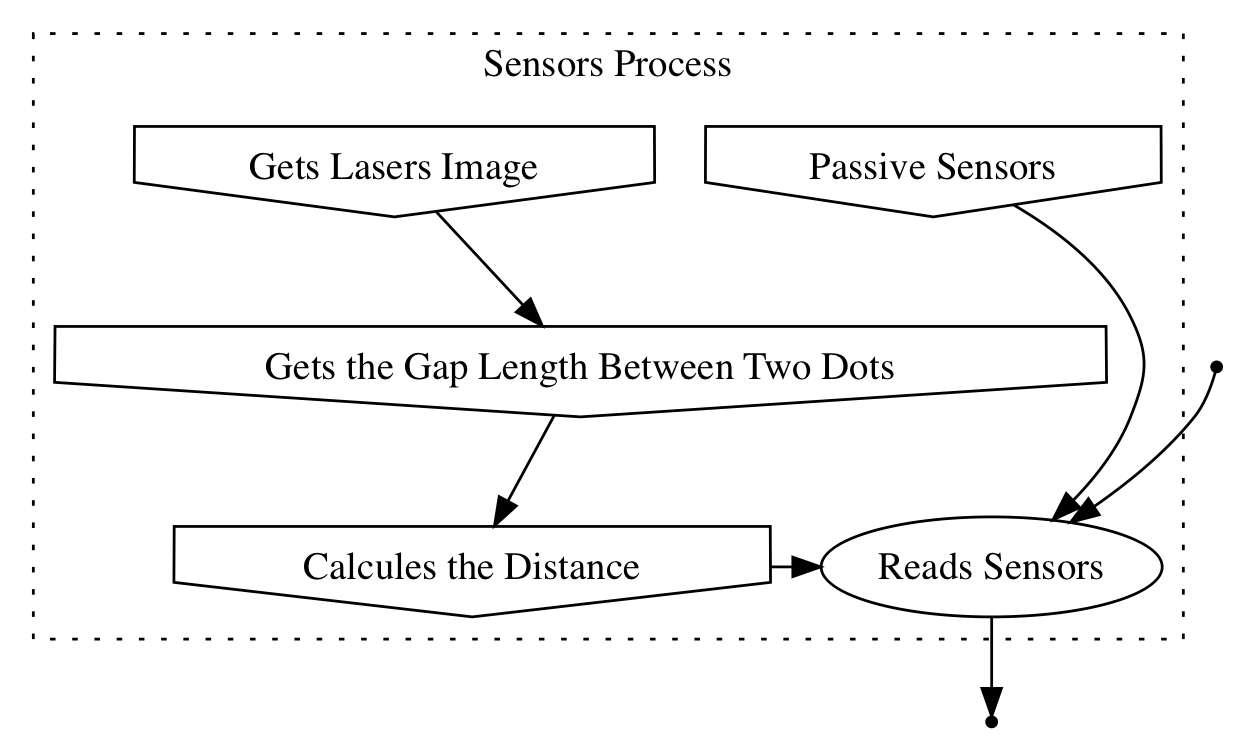
\includegraphics[width=0.8\textwidth]{img/graph_wearable3_b.png}
            \caption{Exemplificação de um grafo de chamada para o exemplo.}
            \label{fig:graph_w3_a}
         \end{figure}
         
         Já o Algoritmo~\ref{alg:wearable3_main} é representado pelo grafo da Figura~\ref{fig:graph_w3_b}.
         Constitui-se do processo principal na qual invoca o procedimento de leitura de sensores.
         Como este é basicamente para controle, nele ordena-se os passos de leitura, exibição e envio dos dados para uma nuvem, caso o dispositivo permaneça ligado neste processo.
         O módulo de leitura de sensores exibido no canto esquerdo da Figura~\ref{fig:graph_w3_b} simplifica o processo da Figura~\ref{fig:graph_w3_a}, já explicada.
         
         \begin{figure}[h] \centering
            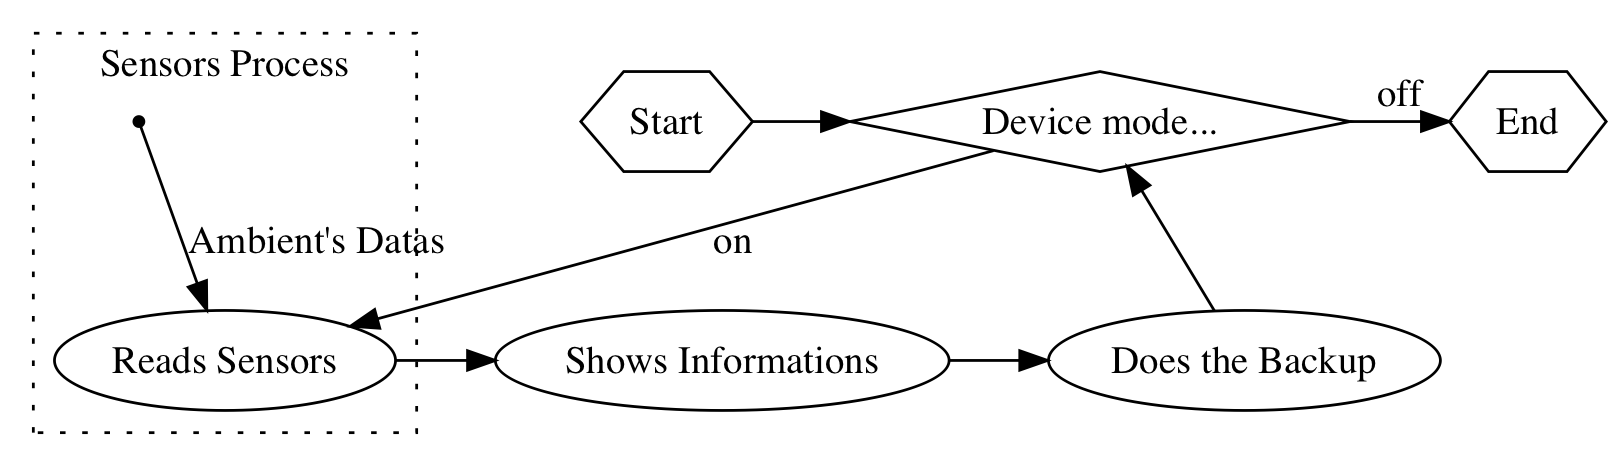
\includegraphics[width=1\textwidth]{img/graph_wearable3.png}
            \caption{Exemplificação de um grafo de chamada para o exemplo.}
            \label{fig:graph_w3_b}
         \end{figure}
         

      \paragraph{Análises de Síntese}
         Idem ao processo das seções anteriores, na qual realiza uma visão do projeto com os candidatos apresentados pelas ferramentas e sintetiza-os a fim de avaliar suas características de funcionamento.
         
      \paragraph{\textit{Solver}}
         Idem às análises anteriores (Seções~\ref{sec:hip1} e \ref{sec:hip2}).

   
   
   
   
   
   
   
   
   
   